\documentclass[a4paper, 14pt]{extarticle}%тип документа
\date{}

%%%Библиотеки
	%\usepackage[warn]{mathtext}	
	\usepackage[T2A]{fontenc} % кодировка
	\usepackage[utf8]{inputenc} % кодировка исходного текста
	\usepackage[english,russian]{babel} % локализация и переносы
	\usepackage{caption}
	\usepackage{listings}
	\usepackage{amsmath,amsfonts,amssymb,amsthm,mathtools}
	\usepackage{wasysym}
	\usepackage{graphicx}%Вставка картинок правильная
	\usepackage{float}%"Плавающие" картинки
	\usepackage{wrapfig}%Обтекание фигур (таблиц, картинок и прочего)
	\usepackage{fancyhdr} %загрузим пакет
	\usepackage{lscape}
	\usepackage{xcolor}
	\usepackage[normalem]{ulem}
	\usepackage{hyperref}

%%%Конец библиотек


\usepackage{graphicx}
\usepackage{cmap}
\usepackage[T2A]{fontenc}
\usepackage[utf8]{inputenc}

%%\renewcommand{\footrulewidth}{ .0em }
\usepackage[english,russian]{babel}
\usepackage{multirow} % Слияние строк в таблице


%Русский язык
\usepackage[T2A]{fontenc} %кодировка
\usepackage[utf8]{inputenc} %кодировка исходного кода
\usepackage[english,russian]{babel} %локализация и переносы

%Таблицы
%\usepackage[table,xcdraw]{xcolor}
%\usepackage{booktabs}

%Математика
\usepackage{amsmath, amsfonts, amssymb, amsthm, mathtools}

%отступы
\usepackage[left=2cm,right=2cm,top=2cm,bottom=3cm,bindingoffset=0cm]{geometry}

%Вставка картинок
\usepackage{graphicx}
\usepackage{wrapfig, caption}
\graphicspath{}
\DeclareGraphicsExtensions{.pdf,.png,.jpg, .jpeg}
\newcommand\ECaption[1]{%
     \captionsetup{font=footnotesize}%
     \caption{#1}}

%Таблицы
%\usepackage[table,xcdraw]{xcolor}
%\usepackage{booktabs}

%Графики
\usepackage{pgfplots}
\pgfplotsset{compat=1.9}
\usepackage[english,russian]{babel}
\usepackage{multirow} % Слияние строк в таблице



\newcommand
{\un}[1]
{\ensuremath{\text{#1}}}

%%%Настройка ссылок
	\hypersetup
	{
		colorlinks=true,
		linkcolor=blue,
		filecolor=magenta,
		urlcolor=blue
	}
%%%Конец настройки ссылок

%%%Настройка колонтитулы
	\pagestyle{fancy}
	\fancyhead{}
	\fancyhead[L]{Лабораторная работа}
	\fancyhead[R]{Талашкевич Даниил, группа Б01-009}
	\fancyfoot[C]{\thepage}
%%%конец настройки колонтитулы\
\begin{document}

%%%Начало титульника
\begin{titlepage}

	\newpage
	\begin{center}
		\normalsize Московский физико-технический институт \\(госудраственный 			университет)
	\end{center}

	\vspace{6em}

	\begin{center}
		\Large Лабораторная работа по РТ цепям\\
	\end{center}

	\vspace{1em}

	\begin{center}
		\large \textbf{Длинные цепи [23]}
	\end{center}

	\vspace{2em}

	\begin{center}
		\large Талашкевич Даниил Александрович\\
		Группа Б01-009
	\end{center}

	\vspace{\fill}

	\begin{center}
	Долгопрудный \\2021
	\end{center}
	
\end{titlepage}
%%%Конец Титульника



%%%Настройка оглавления и нумерации страниц
	\thispagestyle{empty}
	\newpage
	\tableofcontents
	\newpage
	\setcounter{page}{1}
%%%Настройка оглавления и нумерации страниц


\section{Исследование параметров линии}

Так как нет возможности собрать плату и измерить её параметры, выполнение этого пункта пропускаю.

\section{Исследование переходных процессов}

Исследования проводим в режиме $Transient MicroCap$, с подготовленной моделью (файл $TLine.cir$), который содержит длинную линию с волновым сопротивлением $w = 50$ Ом, без потерь, время распространения $\tau=\frac{l}{w}=10$ нс. Линия питается от источника единичного перепада напряжения $V=1$ В.

Наблюдаются напряжения в узлах $e, u$ на входе и выходе линии (переменные $v(e), v(u))$ и входной/выходной токи $i(s) / i(l)$ через виртуальные резисторы $s, l$ с нулевыми сопротивлениями.

В этой модели (файле) Подготовлен вывод графиков амплитуд падающей волны на входе $A(0, t)=\frac{v(e)+50 * i(s)}{2}$ и выходе $A(l, t)=\frac{v(u)+50 * i(l)}{2}($ плот 1$)$, амплитуд отраженной волны на входе $B(0, t)=\frac{v^{2}(e)-50 * i(s)}{2}$ и выходе $B(l, t)=\frac{v(u)-50 * i(l)}{2}($ плот 2$)$, напряжений на входе и выходе $v(e), v(u)$ (плот 3$)$ и токов на входе и выходе $50 * i(s), 50 * i(l)$ (плот 4). 

Временной диапазон графиков выбран равным $20 \tau (\tau = 10$ нс). 


\subsection{Согласованная линия}

На схеме установим $R_{s}=R_{l}=50$ Ом, и выведем графики (через меню $Analisys/Transient/Run$). Проанализируем графики амплитуды падаюшей волны, напряжений и токов. А так же, измерив по графикам установившиеся значения $v(u)$ и $i(l) w$, убедимся в том, что источник отдает в нагрузку предельную мощность:

$P=v(u) i(l)=\frac{V^{2}}{4 R_{s}}, V=1 \mathrm{~B}:$

\[P w=v(u) i(l) w=\frac{V^{2}}{4 R_{s}} w=0,25 .\]

\subsubsection{Выполнение}

\begin{figure}[h!]
			\centering
			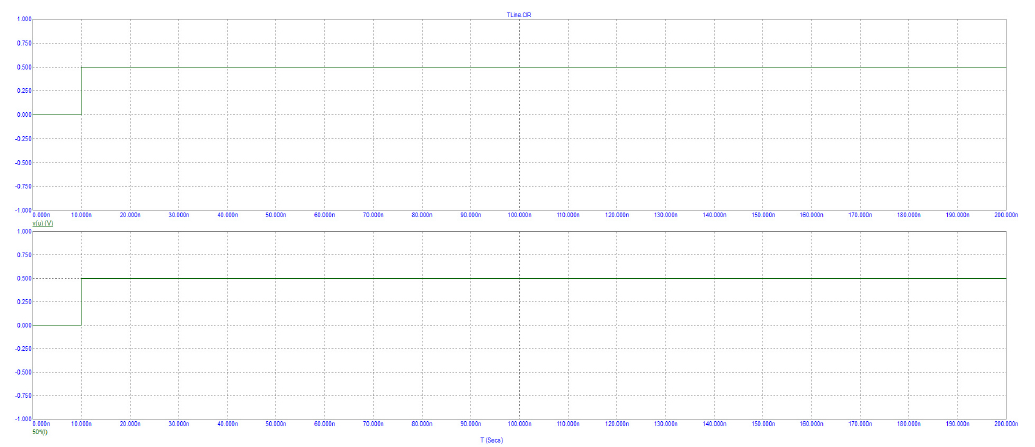
\includegraphics[width=1.1\linewidth]{./graphs/1.jpg}
			\caption{согласованная линия, 1}
			\label{1.1}
\end{figure}

\newpage

\subsubsection{Полученные результаты}

Измерянные значения:

\[ v(u) = 0,5 \text{В}\  i(l) = 0,01 \text{А} ,\]
по ним получаем: 

\[ P=v(u)i(l)=0,005Вт= \frac{V^2}{4R_s} = 1В. \]

Отсюда можно сделать вывод, что формула верна.

\subsection{Рассогласованный источник}

Варьированием установим $R_{s}=\frac{w}{3}\left[\rho_{s}=\frac{R_{s}-w}{R_{s}+w}=-\frac{1}{2}\right]$. ($Transient/Stepping$ - [$From,To|StepValue$ $]=[50 / 3,50 / 3 \mid 1])$. Теперь пересчитаем графики по $Transient/Run$. И, измерив установившиеся значения $v(u)$ и $i(l) w$, проверим, что отдаваемая в нагрузку мощность $P$ меньше мощности источника в $\left(1-\rho_{s}^{2}\right)$ раз, т.е.:

\[
P w=v(u) i(l) w=\frac{V^{2}}{4 R_{s}} w\left(1-\rho_{s}^{2}\right)=0.75\left(1-\frac{1}{4}\right)=0.5625 .
\]

Повторим все это при $R_{s}=3 w\left[\rho_{s}=\frac{R_{s}-w}{R_{s}+w}=+\frac{1}{2}\right]$. Проверим, что

\[
P w=v(u) i(l) w=\frac{V^{2}}{4 R_{s}} w\left(1-\rho_{s}^{2}\right)=\frac{0.25}{3}\left(1-\frac{1}{4}\right)=0.0625 .
\]

\subsubsection{Выполнение}

Установим $R_{S}=\frac{\omega}{3} \text{ Ом} ,\ \omega=50 \text{ Ом},\ \rho_{S}=\frac{R_{S}-\omega}{R_{S}+\omega}=-\frac{1}{2}$. 


\begin{figure}[h!]
			\centering
			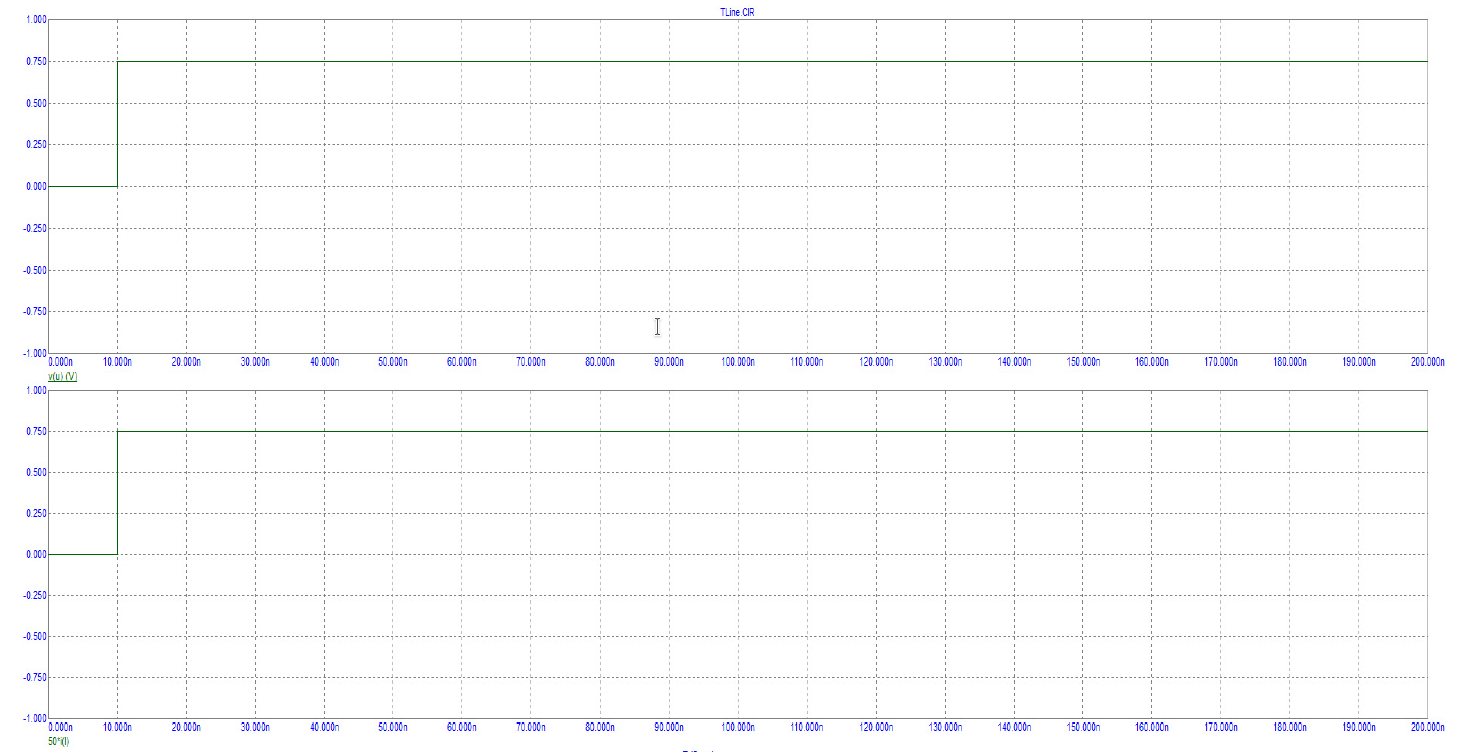
\includegraphics[width=1.1\linewidth]{./graphs/2.jpg}
			\caption{Рассогласованный источник, 1}
			\label{2.1}
\end{figure}

Повторим те же измерения при $R_{S}=3 \omega$, $\rho_{S}=\frac{1}{2}$:


\begin{figure}[h!]
			\centering
			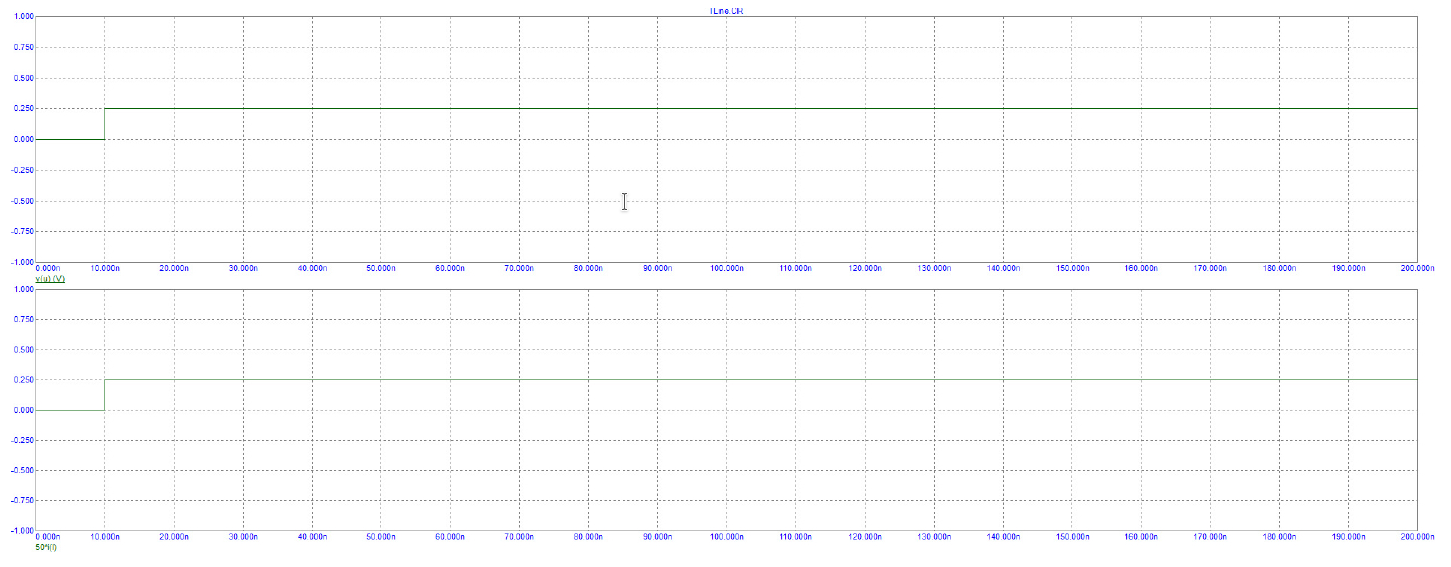
\includegraphics[width=1.1\linewidth]{./graphs/3.jpg}
			\caption{Рассогласованный источник, 2}
			\label{2.2}
\end{figure}

\subsubsection{Полученные результат}

\[v(u)=0,75 \text{B},\ i(l) \omega=0,75\text{B}\]

\[ P \omega=v(u) i(l) \omega=0,5625=\frac{V^{2}}{4 R_{S}} \omega\left(1-\rho_{S}^{2}\right),
\]

что говорит о справедливости утверждения о том, что отдаваемая в нагрузку мозность $P$ меньше мощности источника в $(1 - \rho_{S}^2) \text{ раз}.$

Полученный значения, при $R_{S}=3 \omega$, $\rho_{S}=\frac{1}{2}$:

\[v(u)=0,25 \text{B},\ i(l) \omega=0,25\text{B}\]

\[ P \omega=v(u) i(l) \omega=0,0625=\frac{V^{2}}{4 R_{S}} \omega\left(1-\rho_{S}^{2}\right),
\]

аналогично следует вывод о том, что мощность, отдаваемая в нагрузку меньше мощности источника в $(1 - \rho_{S}^2) \text{ раз}.$

\subsection{Рассогласованная нагрузка}

Установим варьированием $R_{l}=\frac{w}{3}\left[\rho_{l}=-\frac{1}{2}\right]$. Выясним характер переходных процессов, а так же измерим установившиеся значения амплитуд волн, напряжений и токов.

Повторим все наблюдения при $R_{l}=0\left[\rho_{l}=-1\right], R_{l}=3 w$ $\left[\rho_{l}=+\frac{1}{2}\right], R_{l}=50 k \simeq \infty\left[\rho_{l}=+1\right]$.

\subsubsection{Выполнение}

\[R_l =\frac{w}{3},\  v(u)=0,25 \text{B},\ i(l)w =0,75 \text{В} :\]

\begin{figure}[h!]
			\centering
			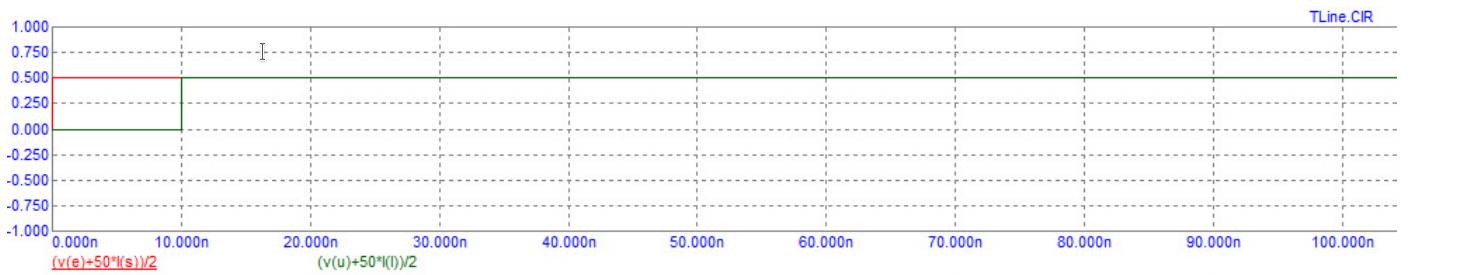
\includegraphics[width=1.1\linewidth]{./graphs/4.jpg}
			%\caption{Рассогласованная нагрузка, 1}
			\label{3.1.1}
\end{figure}

\newpage

\begin{figure}[h!]
			\centering
			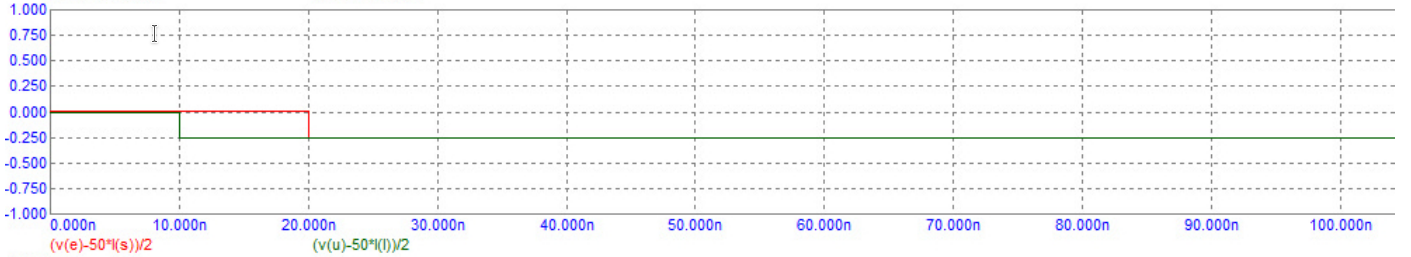
\includegraphics[width=1.1\linewidth]{./graphs/5.jpg}
			%\caption{Рассогласованная нагрузка, 1}
			\label{3.1.2}
\end{figure}


\begin{figure}[h!]
			\centering
			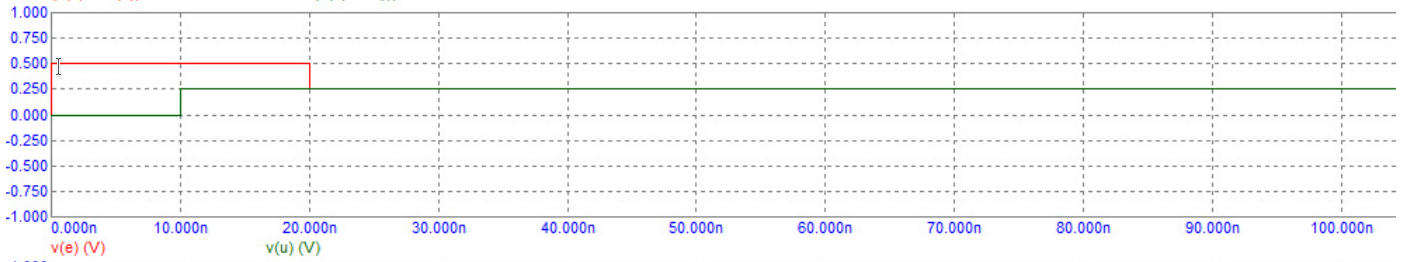
\includegraphics[width=1.1\linewidth]{./graphs/6.jpg}
			%\caption{Рассогласованная нагрузка, 1}
			\label{3.1.3}
\end{figure}


\begin{figure}[h!]
			\centering
			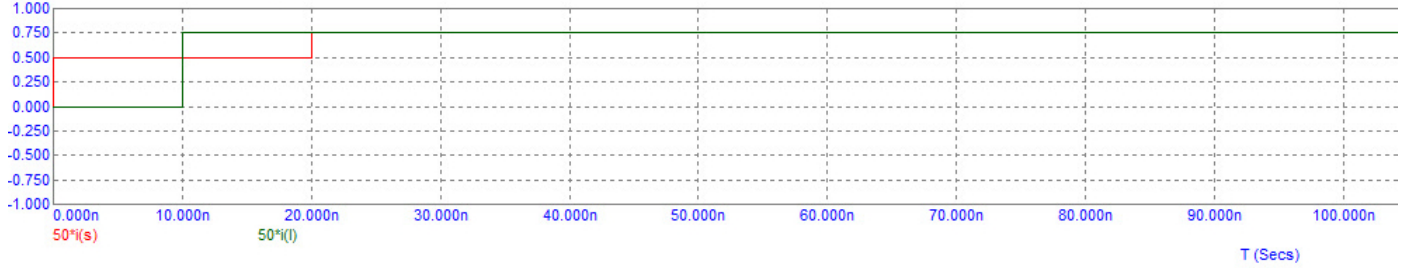
\includegraphics[width=1.1\linewidth]{./graphs/7.jpg}
			\caption{Рассогласованная нагрузка, 1}
			\label{3.1.4}
\end{figure}

\[R_l =3w,\  v(u)=0,75 \text{B},\ i(l)w =0,25 \text{В} :\]

\begin{figure}[h!]
			\centering
			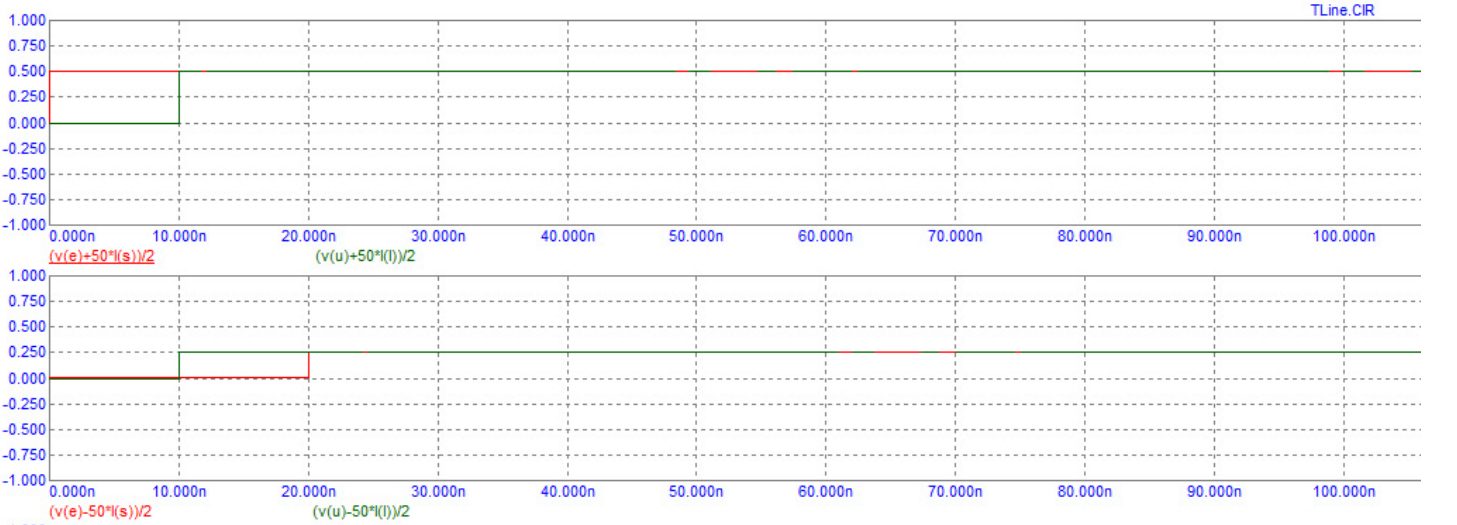
\includegraphics[width=1.1\linewidth]{./graphs/8.jpg}
			%\caption{Рассогласованная нагрузка, 2}
			\label{3.2.1}
\end{figure}


\begin{figure}[h!]
			\centering
			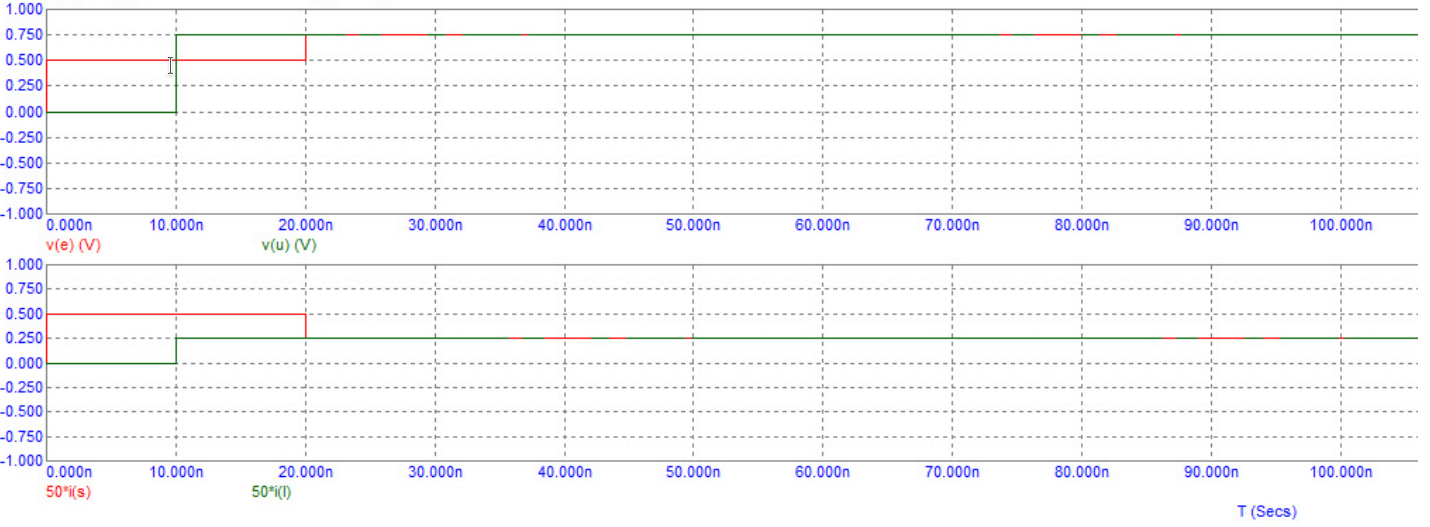
\includegraphics[width=1.1\linewidth]{./graphs/9.jpg}
			\caption{Рассогласованная нагрузка, 2}
			\label{3.2.2}
\end{figure}

\[R_l =0w,\  v(u)=0,00 \text{B},\ i(l)w =1,00 \text{В} :\]

\begin{figure}[h!]
			\centering
			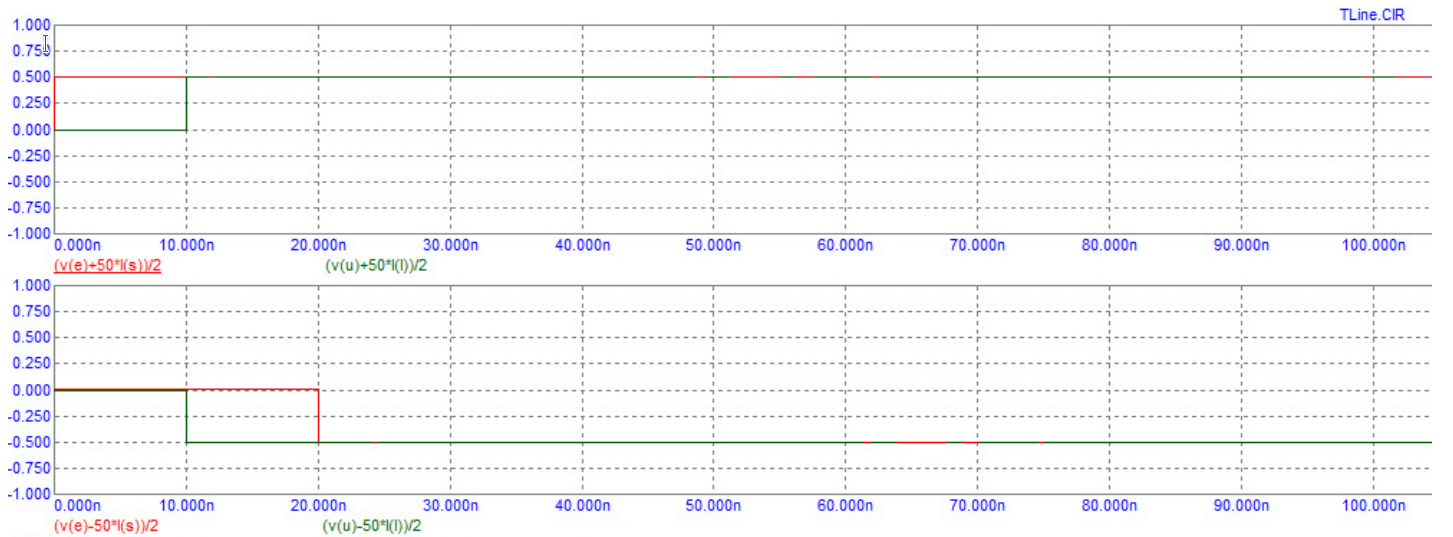
\includegraphics[width=1.1\linewidth]{./graphs/10.jpg}
			%\caption{Рассогласованная нагрузка, 2}
			\label{3.3.1}
\end{figure}

\newpage

\begin{figure}[h!]
			\centering
			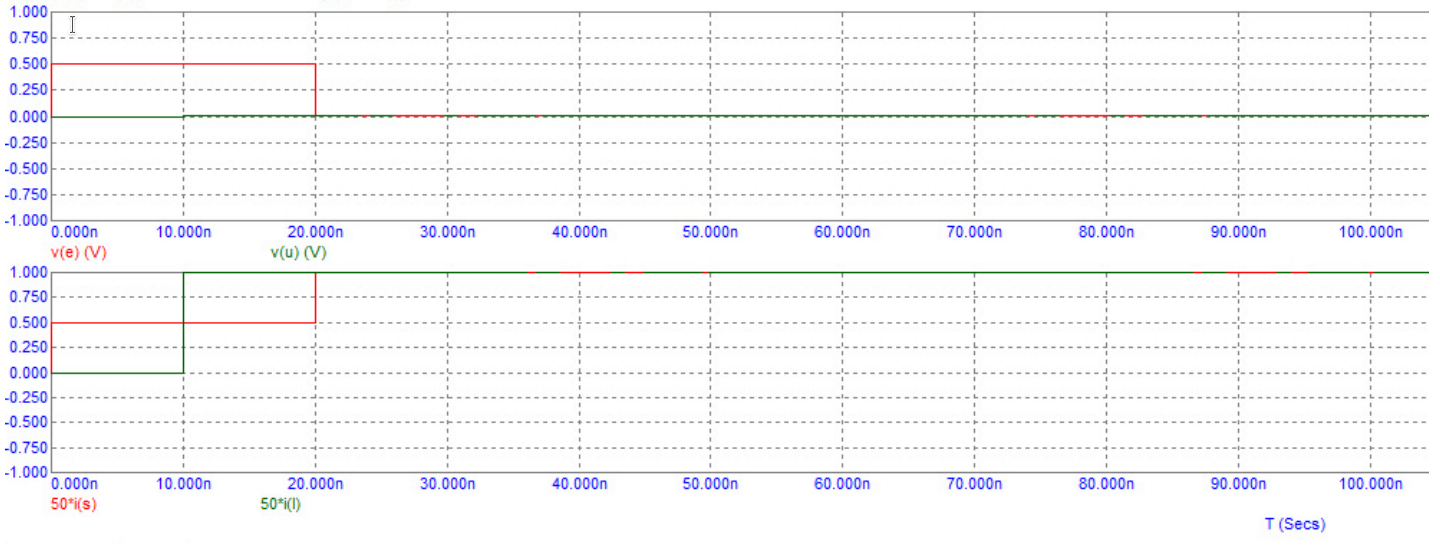
\includegraphics[width=1.1\linewidth]{./graphs/11.jpg}
			\caption{Рассогласованная нагрузка, 3}
			\label{3.3.2}
\end{figure}

\[R_l =\infty,\  v(u)=1,00 \text{B},\ i(l)w =0,00 \text{В} :\]

\begin{figure}[h!]
			\centering
			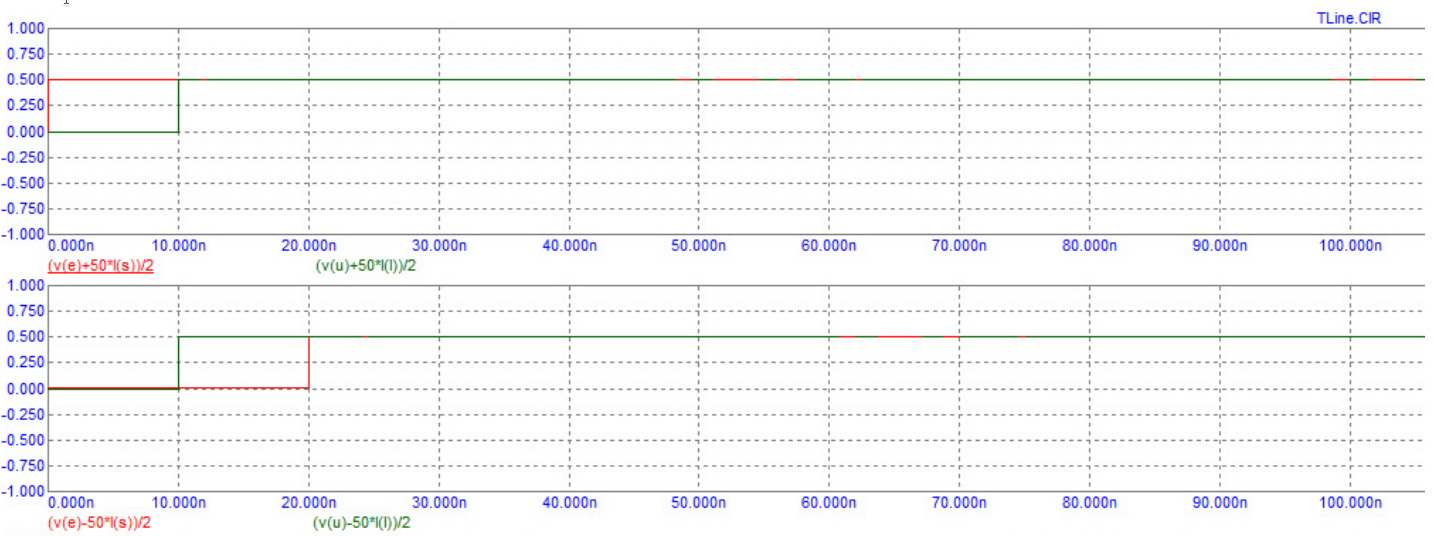
\includegraphics[width=1.1\linewidth]{./graphs/12.jpg}
			%\caption{Рассогласованная нагрузка, 2}
			\label{3.4.1}
\end{figure}

\newpage

\begin{figure}[h!]
			\centering
			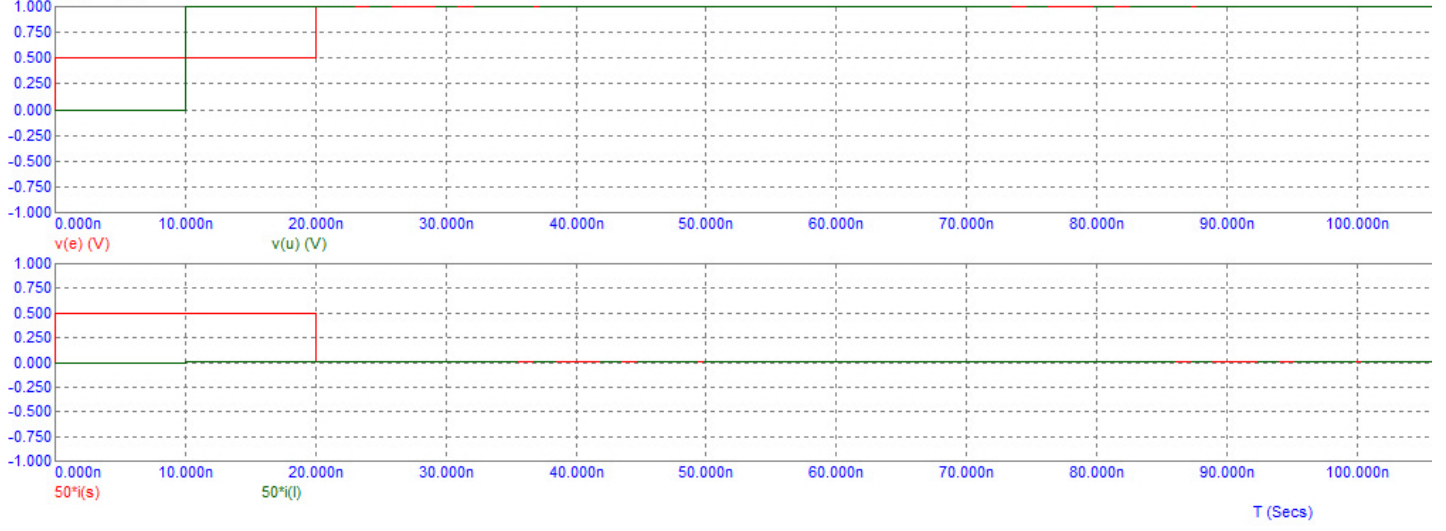
\includegraphics[width=1.1\linewidth]{./graphs/13.jpg}
			\caption{Рассогласованная нагрузка, 4}
			\label{3.4.2}
\end{figure}

\subsubsection{Полученные результаты}

Из графиков установившиеся значения амплитуд волн, напряжений и токов:

\[R_l =\frac{w}{3};\  v(u)=0,25 \text{B};\ i(l)w =0,75 \text{В} :\]
\[  A = 0,5 \text{B};\ B = -0,250 \text{B};\ v = 0,250 \text{B};\ i(l)w = 0,750 \text{B}.\]

\[R_l =3w;\  v(u)=0,75 \text{B};\ i(l)w =0,25 \text{В} :\]
\[  A = 0,5 \text{B};\ B = 0,250 \text{B};\ v = 0,750 \text{B};\ i(l)w = 0,250 \text{B}.\]

\[R_l =0w;\  v(u)=0,00 \text{B};\ i(l)w =1,00 \text{В} :\]
\[  A = 0,5 \text{B};\ B = -0,500 \text{B};\ v = 0,000 \text{B};\ i(l)w = 1,000 \text{B}.\]

\[R_l =\infty;\  v(u)=1,00 \text{B};\ i(l)w =0,00 \text{В} :\]
\[  A = 0,5 \text{B};\ B = 0,500 \text{B};\ v = 1,000 \text{B};\ i(l)w = 0,000 \text{B}.\]


\subsection{Рассогласованный источник и нагрузка}

Установим на схеме $R_{s}=50 / 3\left[\rho_{s}=-\frac{1}{2}\right] .$ Установив варьированием $R_{l}=0\left[\rho_{l}=-1\right], \rho_{s} \rho_{l}=\frac{1}{2}$, изобразим полученные графики. По ним убедимся, что амплитуда падающей волны нарастает как последовательность частичных сумм прогрессии:


\[
A=\frac{w}{w+R_{s}}\left(1+\rho_{s} \rho_{l}+\left(\rho_{s} \rho_{l}\right)^{2}+\ldots\right)=\frac{3}{4}\left(1+\frac{1}{2}+\frac{1}{4}+\frac{1}{8}+\ldots\right) .
\]

Как итог, объясним ход графиков амплитуд волн, напряжений и токов и измерим установившиеся значения.

Повторим наблюдения при $R_{l}=50 k \simeq \infty\left[\rho_{l}=1\right], \rho_{s} \rho_{l}=-\frac{1}{2}$ : 

\[A=\frac{w}{w+R_{s}}\left(1+\rho_{s} \rho_{l}+\left(\rho_{s} \rho_{l}\right)^{2}+\ldots\right)=\frac{3}{4}\left(1-\frac{1}{2}+\frac{1}{4}-\frac{1}{8}+\ldots\right)\]

Установим на схеме $R_{s}=50 * 3\left[\rho_{s}=+\frac{1}{2}\right]$ и повторим наблюдения при $R_{l}=0\left[\rho_{l}=-1\right]$ :

\[A=\frac{w}{w+R_{s}}\left(1+\rho_{s} \rho_{l}+\left(\rho_{s} \rho_{l}\right)^{2}+\ldots\right)=\frac{1}{4}\left(1-\frac{1}{2}+\frac{1}{4}-\frac{1}{8}+\ldots\right)\]

и $R_{l}=50 k \simeq \infty\left[\rho_{l}=1\right]$ :

\[A=\frac{w}{w+R_{s}}\left(1+\rho_{s} \rho_{l}+\left(\rho_{s} \rho_{l}\right)^{2}+\ldots\right)=\frac{1}{4}\left(1+\frac{1}{2}+\frac{1}{4}+\frac{1}{8}+\ldots\right) .\]

Установим на схеме $R_{s}=0\left[\rho_{s}=-1\right]$ (предельно сильное рассогласование на источнике) и повторим наблюдения при

\[
\begin{aligned}
R_{l}=50 k, &\left[\rho_{l}=1\right] \quad \Rightarrow A=(1-1+1-1+\ldots), \\
R_{l}=500, \quad\left[\rho_{l}=0.8\right] \quad & \Rightarrow A=\left(1-\rho_{l}+\rho_{l}^{2}-\rho_{l}^{3}+\ldots\right), \\
R_{l}=0, \quad\left[\rho_{l}=1\right] \quad & \Rightarrow A=(1+1+1+1+\ldots), \\
R_{l}=5, \quad\left[\rho_{l}=-0.8\right] \quad & \Rightarrow A=\left(1+\rho_{l}+\rho_{l}^{2}+\rho_{l}^{3}+\ldots\right).
\end{aligned}
\]

\subsubsection{Выполнение}

\[R_{S}=\frac{50}{3},\ \rho_{S}=-\frac{1}{2},\  R_{l}=0,\ \rho_{l}=-1,\ \rho_{S} \rho_{l}=\frac{1}{2},\]

\[ \text{где }A=\frac{\omega}{\omega+R_{S}}\left(1+\rho_{S} \rho_{l}+\left(\rho_{S} \rho_{l}\right)^{2}+\ldots\right)=\frac{3}{4}\left(1+\frac{1}{2}+\frac{1}{4}+\frac{1}{8}+\ldots\right) :\]

\newpage

\begin{figure}[h!]
			\centering
			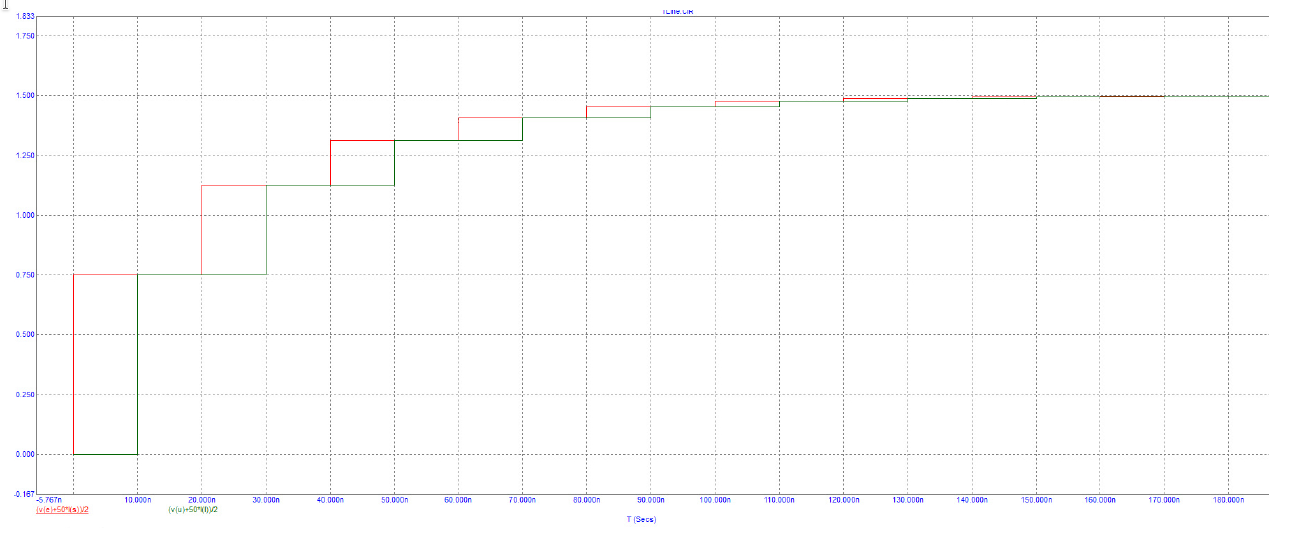
\includegraphics[width=1.1\linewidth]{./graphs/14.jpg}
			\caption{Рассогласованный источник и нагрузка, 1}
			\label{4.1}
\end{figure}

\[R_{S}=\frac{50}{3},\ \rho_{S}=-\frac{1}{2},\  R_{l}=50k \simeq \infty,\ \rho_{l}=1,\ \rho_{S} \rho_{l}=-\frac{1}{2},\]

\[ \text{где }A=\frac{\omega}{\omega+R_{S}}\left(1+\rho_{S} \rho_{l}+\left(\rho_{S} \rho_{l}\right)^{2}+\ldots\right)=\frac{3}{4}\left(1-\frac{1}{2}+\frac{1}{4}-\frac{1}{8}+\ldots\right) :\]

\begin{figure}[h!]
			\centering
			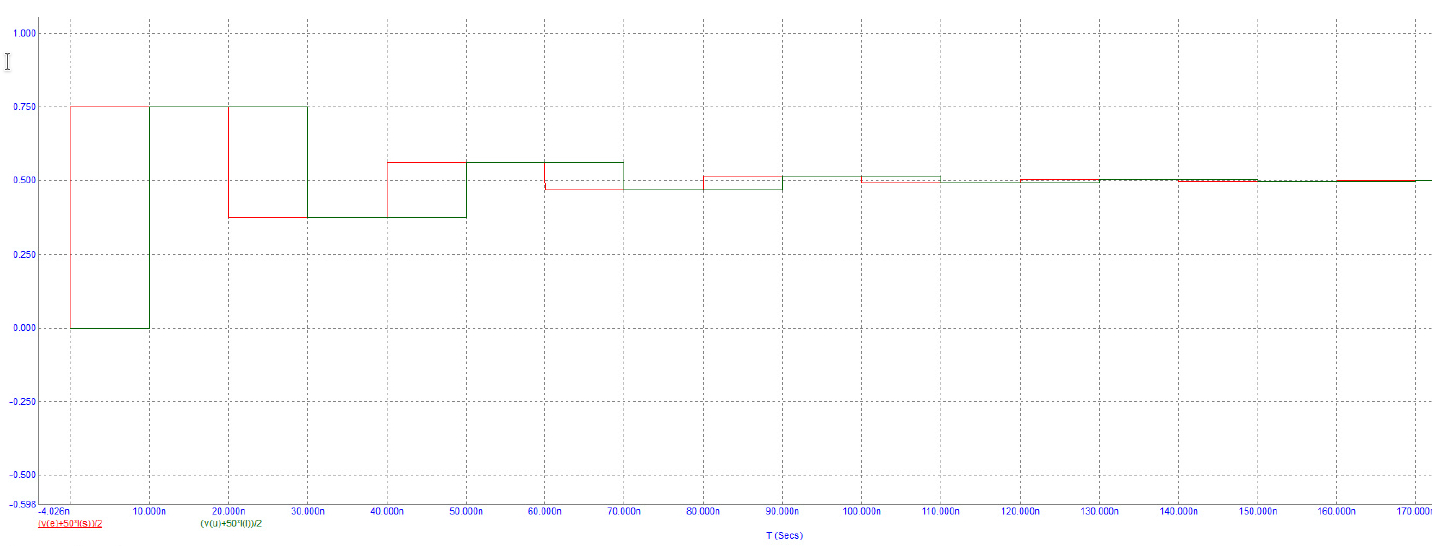
\includegraphics[width=1.1\linewidth]{./graphs/15.jpg}
			\caption{Рассогласованный источник и нагрузка, 2}
			\label{4.2}
\end{figure}

Установим $R_{S}=0,\ \rho_{S}=-1$ (предельно сильное рассогласование на источнике) и повторим наши наблюдения при

\[ R_{l}=50 k, \left[\rho_{l}=1\right] \ \Rightarrow A=(1-1+1-1+\ldots) : \]

\begin{figure}[h!]
			\centering
			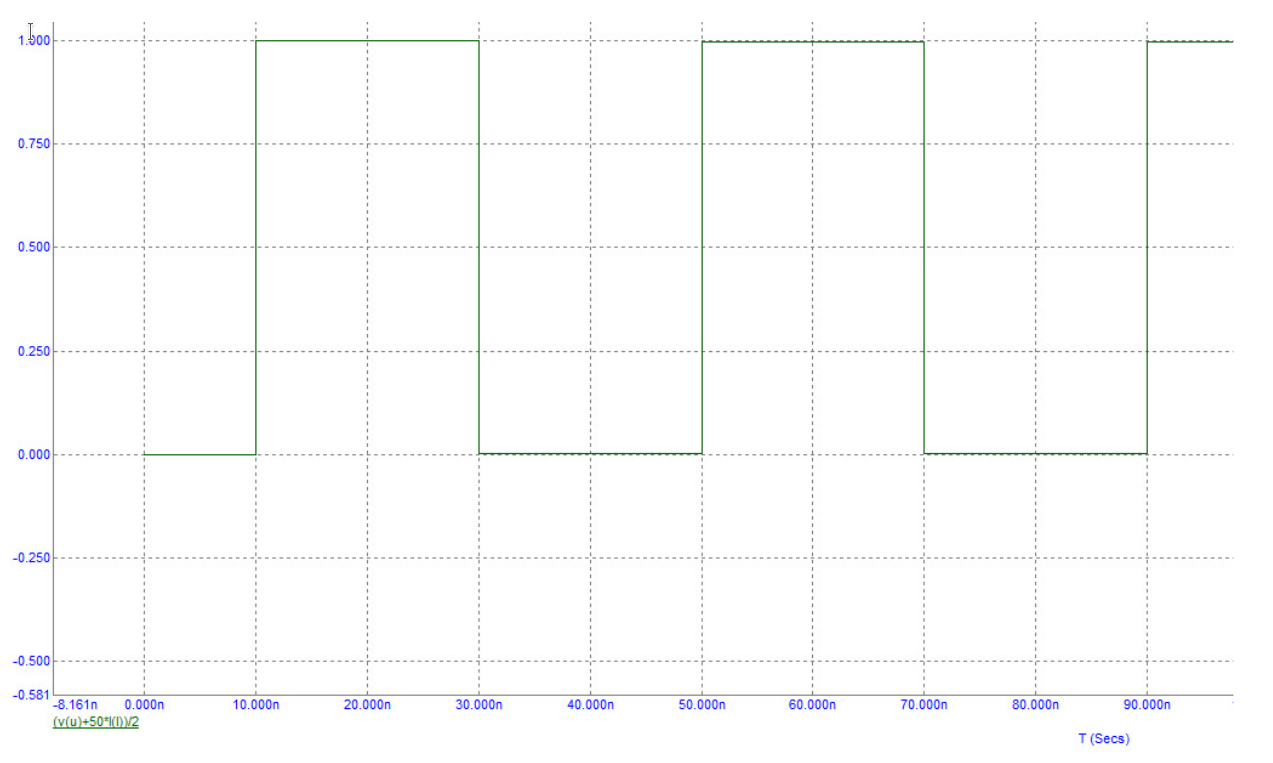
\includegraphics[width=1.1\linewidth]{./graphs/16.jpg}
			\caption{Рассогласованный источник и нагрузка, 3}
			\label{4.3}
\end{figure}

\[R_{l}=500,\ \left[\rho_{l}=0.8\right] \ \Rightarrow A=\left(1-\rho_{l}+\rho_{l}^{2}-\rho_{l}^{3}+\ldots\right):\]

\begin{figure}[h!]
			\centering
			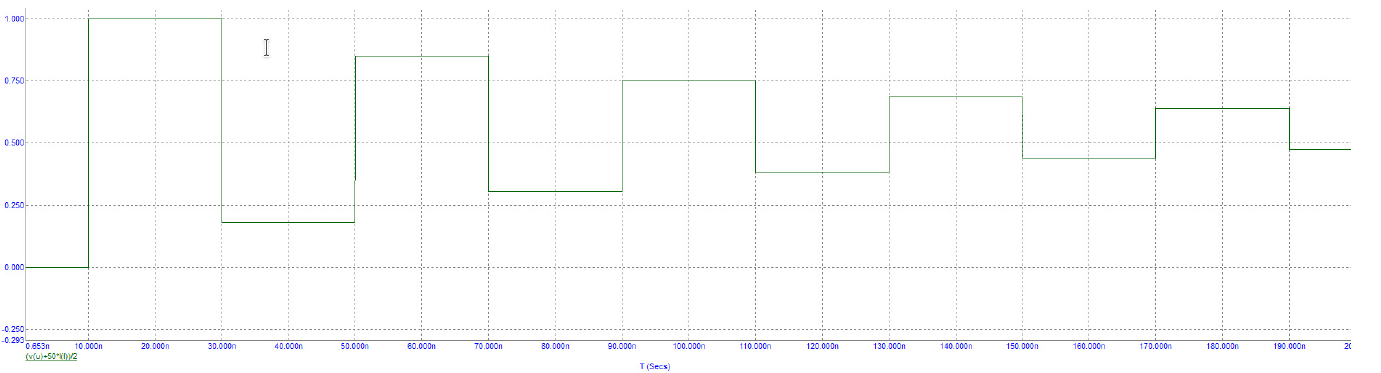
\includegraphics[width=1.1\linewidth]{./graphs/17.jpg}
			\caption{Рассогласованный источник и нагрузка, 4}
			\label{4.4}
\end{figure}

\[R_{l}=0,\ \left[\rho_{l}=1\right] \ \Rightarrow A=(1+1+1+1+\ldots): \]

\newpage

\begin{figure}[h!]
			\centering
			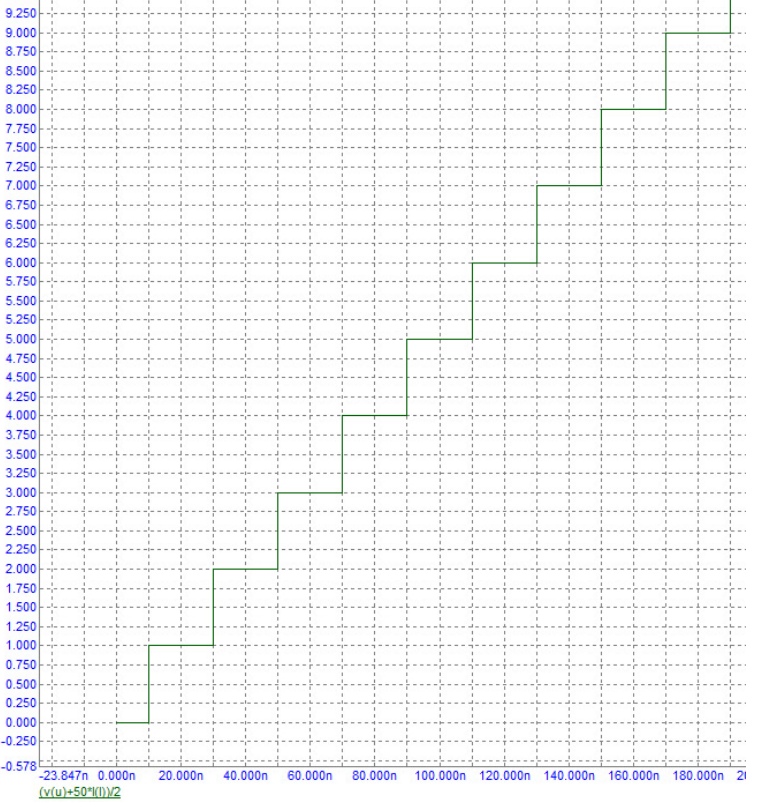
\includegraphics[width=1.1\linewidth]{./graphs/18.jpg}
			\caption{Рассогласованный источник и нагрузка, 5}
			\label{4.5}
\end{figure}

\[R_{l}=5, \ \left[\rho_{l}=-0.8\right] \  \Rightarrow A=\left(1+\rho_{l}+\rho_{l}^{2}+\rho_{l}^{3}+\ldots\right) : \]

\newpage

\begin{figure}[h!]
			\centering
			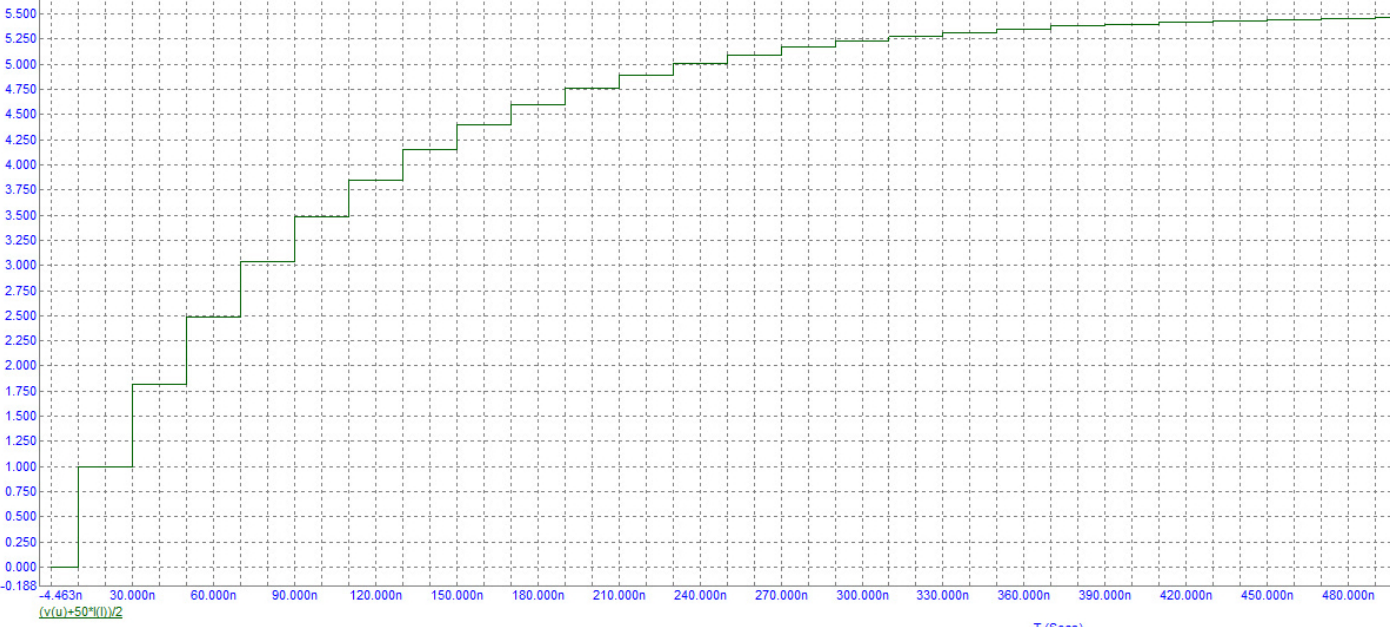
\includegraphics[width=1.1\linewidth]{./graphs/19.jpg}
			\caption{Рассогласованный источник и нагрузка, 4}
			\label{4.4}
\end{figure}


\subsubsection{Полученные результаты}

Из графиков отлично виден характер нарастания амплитуды падающей волны. И этот характер полностью совпадает с соответствующими последовательностями частичных сумм для амплитуды падающей волны. Получили полное соответствие с теорией.

$\textbf{Установившиеся значения:}$

\[ R_{S}=\frac{50}{3},\ \rho_{S}=-\frac{1}{2},\  R_{l}=0,\ \rho_{l}=-1,\ \rho_{S} \rho_{l}=\frac{1}{2}:\]
\[ A = 1,5 \text{B}.\]

\[R_{S}=\frac{50}{3},\ \rho_{S}=-\frac{1}{2},\  R_{l}=50k \simeq \infty,\ \rho_{l}=1,\ \rho_{S} \rho_{l}=-\frac{1}{2},\]
\[ A = 0,5 \text{B}.\]

\[ R_{l}=50 k, \left[\rho_{l}=1\right] : \]
\[ \text{установившегося значения нет, }A \text{ колебается между 0 | 1 }\text{B}.\]

\[R_{l}=500,\ \left[\rho_{l}=0.8\right] \ \Rightarrow A=\left(1-\rho_{l}+\rho_{l}^{2}-\rho_{l}^{3}+\ldots\right):\]
\[ A = 0,(5) \text{B}.\]

Последний результат теоретически можно проверить следующий образом:

\[ A_{\text{уст}} = \lim_{n \rightarrow \infty} s_n = \frac{b_1}{1 - q} = \frac{1}{1 + 0,8} = 0,(5)\text{B}.\]

Отсюда видно, что значения совпадают.

\[R_{l}=0,\ \left[\rho_{l}=1\right] \ \Rightarrow A=(1+1+1+1+\ldots): \]
\[ \text{установившегося значения нет, }A \text{ дискретно увеличивается на 1}\text{B}.\]

\[R_{l}=5, \ \left[\rho_{l}=-0.8\right] \  \Rightarrow A=\left(1+\rho_{l}+\rho_{l}^{2}+\rho_{l}^{3}+\ldots\right) : \]
\[ A = 5,(5) \text{B}.\]

Полученный результат качественно совпадает с теорией, но полученное значение расходится с теоретическим:

\[ A_{\text{уст}} = \lim_{n \rightarrow \infty} s_n = \frac{b_1}{1 - q} = \frac{1}{1 - 0,8} = 5,0 \text{B}.\]

Видимо при симуляции было выставлено не то значение, по полученному результату можно получить это значение : $\rho_l = 0,(81)$.

\subsection{Емкостная нагрузка}

Установим на схеме $R_{s}=50$ (согласованный источник), $R_{l}=50 k \simeq \infty, C=100$ пФ. Объясним формы графиков переходных процессов. Измерим установившиеся значения амплитуд волн, напряжений и токов. Оценим по графикам постоянную времени $\tau$ экспоненциального переходного процесса и проверить, что $\tau=w C$.

Варьированием установить $R_{s}=50 / 3$, проанализировать графики переходных процессов. Измерить установившиеся значения амплитуд волн, напряжений и токов.

И, наконец, проанализируем графики незатухающего переходного процесса при $R_{s}=0 .$

\subsubsection{Выполнение}

\[ R_{S}=50,\ A=0,5 B,\ v=1 \text{B},\  i \omega=0 \text{B},\ \tau=\omega C = 5 * 10^{-9} \text{c}:\]

\newpage

\begin{figure}[h!]
			\centering
			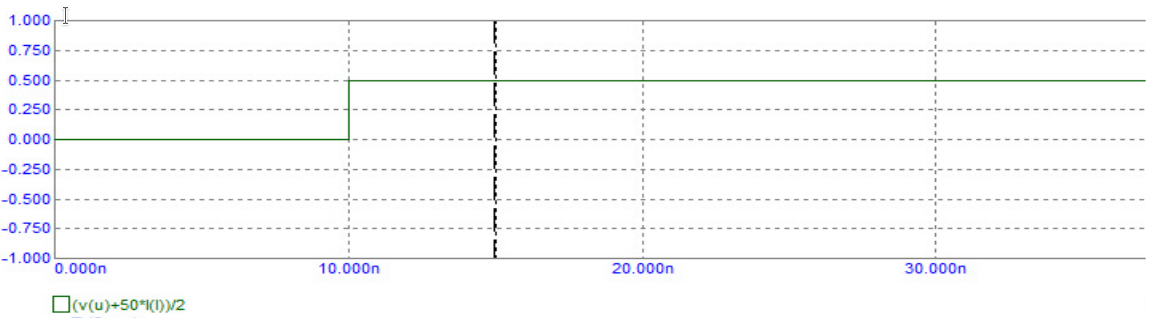
\includegraphics[width=1.1\linewidth]{./graphs/20.jpg}
			\caption{Емкостная нагрузка, 1}
			\label{5.1}
\end{figure}

\begin{figure}[h!]
			\centering
			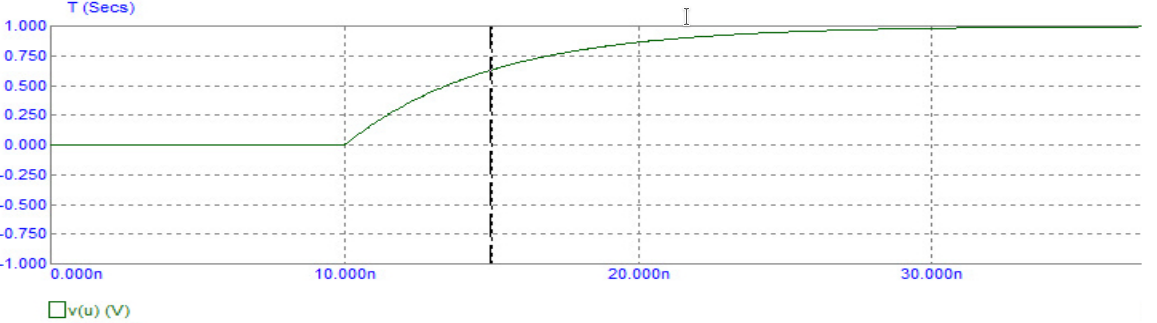
\includegraphics[width=1.1\linewidth]{./graphs/21.jpg}
			\caption{Емкостная нагрузка, 2}
			\label{5.2}
\end{figure}

\begin{figure}[h!]
			\centering
			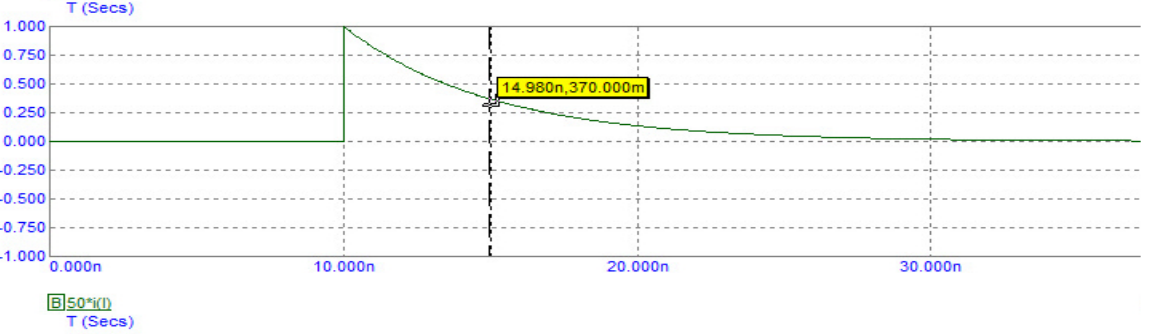
\includegraphics[width=1.1\linewidth]{./graphs/22.jpg}
			\caption{Емкостная нагрузка, 3}
			\label{5.3}
\end{figure}

\[ R_{S}=\frac{50}{3},\ A=0,5 B,\ v=1 \text{B},\  i \omega=0 \text{B}:\]

\newpage

\begin{figure}[h!]
			\centering
			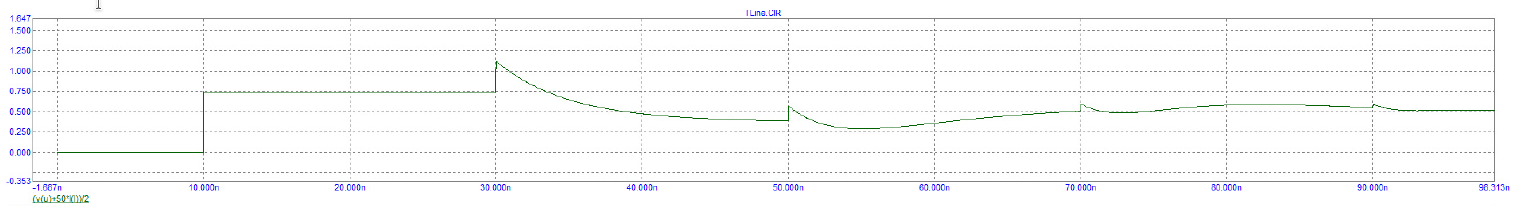
\includegraphics[width=1.1\linewidth]{./graphs/23.jpg}
			\caption{Емкостная нагрузка, 4}
			\label{5.4}
\end{figure}

\begin{figure}[h!]
			\centering
			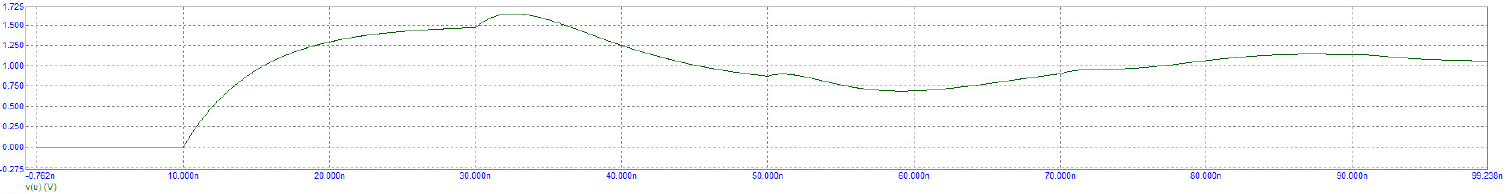
\includegraphics[width=1.1\linewidth]{./graphs/24.jpg}
			\caption{Емкостная нагрузка, 5}
			\label{5.5}
\end{figure}

\begin{figure}[h!]
			\centering
			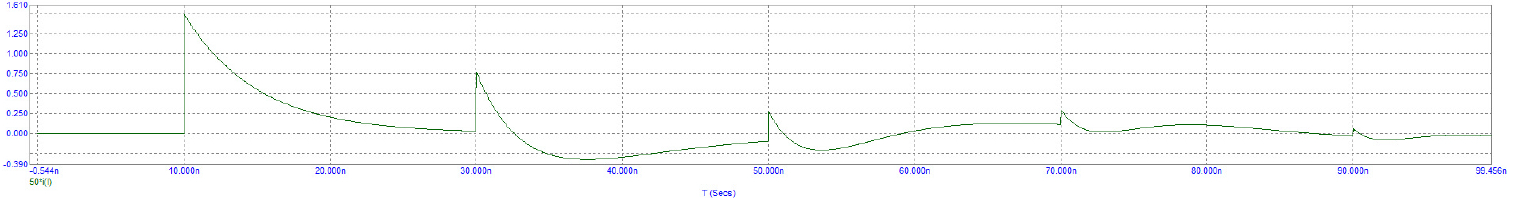
\includegraphics[width=1.1\linewidth]{./graphs/25.jpg}
			\caption{Емкостная нагрузка, 6}
			\label{5.6}
\end{figure}

\[ R_{S}=0,\ A=0,5 B,\ v=1 \text{B},\  i \omega=0 \text{B}:\]

\begin{figure}[h!]
			\centering
			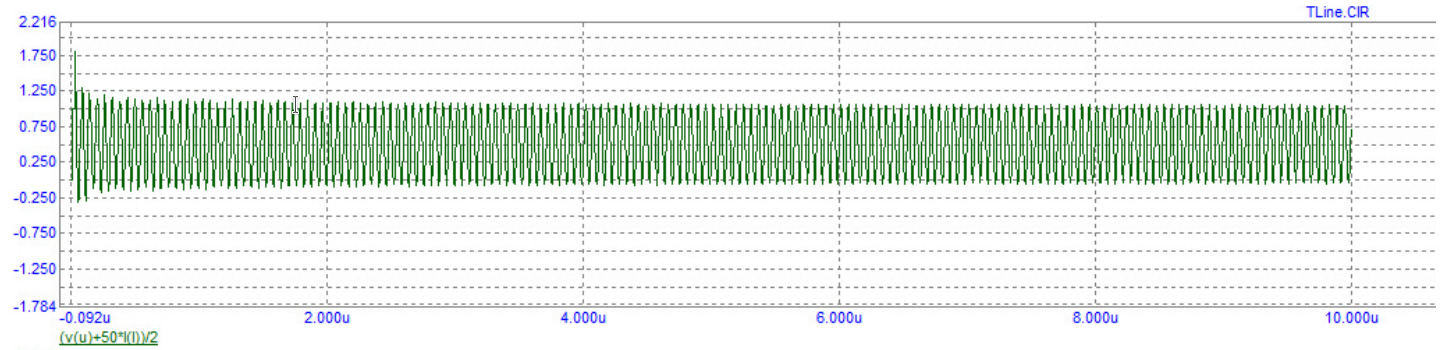
\includegraphics[width=1.1\linewidth]{./graphs/26.jpg}
			\caption{Емкостная нагрузка, 7}
			\label{5.7}
\end{figure}

\newpage 

\begin{figure}[h!]
			\centering
			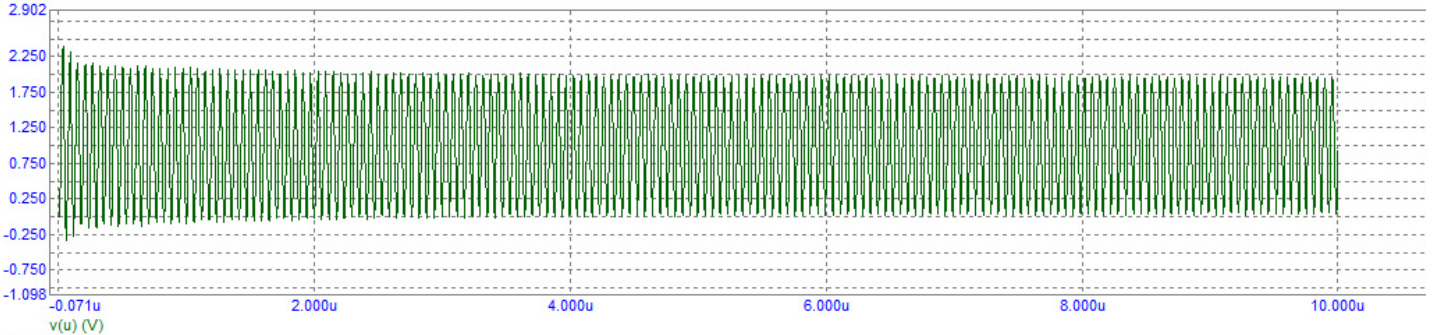
\includegraphics[width=1.1\linewidth]{./graphs/27.jpg}
			\caption{Емкостная нагрузка, 8}
			\label{5.8}
\end{figure}

\begin{figure}[h!]
			\centering
			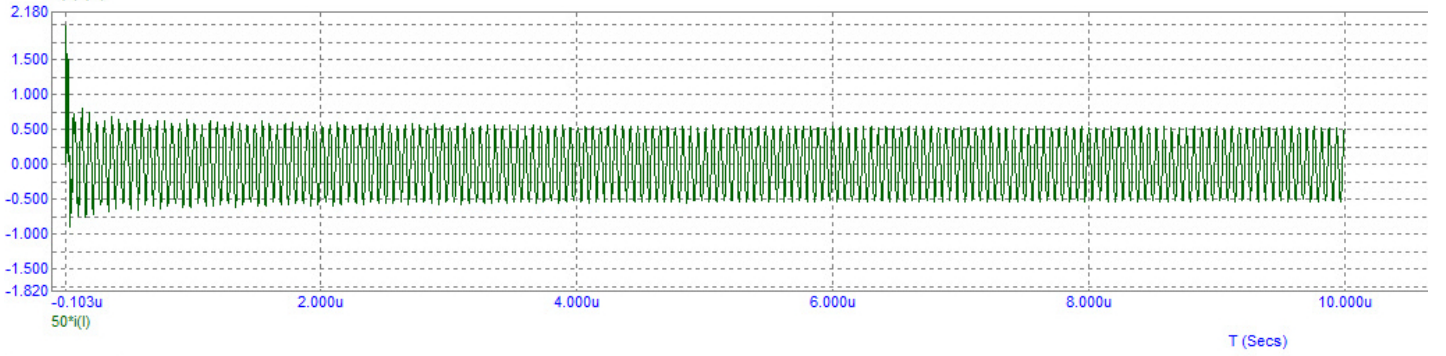
\includegraphics[width=1.1\linewidth]{./graphs/28.jpg}
			\caption{Емкостная нагрузка, 9}
			\label{5.9}
\end{figure}

\subsubsection{Полученные результат}

$\textbf{Установившиеся значения амплитуд волн, напряжений и токов:}$

\[ R_{S}=50\ :\]
\[  A=0,5 B;\ v=1 \text{B};\  i \omega=0 \text{B}\]

Из графика $\ref{5.3}$ видно, что уменьшение на $\simeq 70 \%$ соответствует временному сдвигу примерно в $5 \text{ нс}$, откуда следует вывод, что постоянная времени экспоненциального перехода совпадает с теоретической $\tau = wC$.

$\textbf{Установившиеся значения амплитуд при }R_s = \frac{50}{3}:$

\[ A = 0,5\text{B};\ v = 1\text{B};\ i(l)w = 0\text{B}.\]

$\textbf{Анализ незатухающего переходного процесса при } R_s = 0:$

Как и ожидалось, при $R_{S}=0$ сигнал не будет затухать, а будут лишь наблюдаться колебания около среднего значения.


\section{Литература}

\begin{itemize}

\item Григорьев А.А. Лекции по теории длинных цепец. - М.: МФТИ, $2013 .$

\item Методические указания к работе №$23 (\text{Длинный цепи})$.

\end{itemize}


\end{document}
